\chapter{Chorale harmonization}

% **************************** Define Graphics Path **************************
\ifpdf
    \graphicspath{{Chapter5/Figs/Raster/}{Chapter5/Figs/PDF/}{Chapter5/Figs/}}
\else
    \graphicspath{{Chapter5/Figs/Vector/}{Chapter5/Figs/}}
\fi

\mynote{Talk about how correct harmonization is equivalent to conditioning on
  future hidden state over all possible $\h$ trajectories passing through it.
  Intractable conditioning, so we approximate by neglecting to constrain (i.e.
  don't account for future at all) and instead do teacher forcing. Hope that
  teacher forcing induces the hidden state to go in a reasonable trajectory,
but results show otherwise}

Unlike automatic composition, in harmonization tasks we are given the entire sequence of notes
for one or more parts. As one of the parts is now fixed, the model is no longer able to freely
compose and harmonic deviations from the fixed parts will result in dissonances and conflicting
expectations. This lack of accountability for future expectations is one of the failure modes of our models.
One potential method for mitigating this is bidirectional LSTMs\citep{Graves2005}, which account
for both the future and prior contexts. However, a bidirectional LSTM cannot be sequentially
sampled to perform automatic composition.

\section{Background}

A chorale consists of four parts: soprano, alto, tenor, and bass. Chorale harmonization
involves producing the alto, tenor, and bass parts given a fixed soprany melody. As described
by Walter Piston \citep{piston1978harmony}:

\begin{quote}
  True harmonisation, then, means a consideration of the alternatives in available chords, the reasoned selection of one
  of these alternatives, and the tasteful arrangement of the texture of the added parts with due regard
  for consistency of style
\end{quote}

The Baroque style employed by Bach has specific guidelines
such as disallowing parallel fifths and parallel octaves as well as
considerations for voice leading \citep{piston1978harmony}.

For a music student studying chorale harmonization, a common pedagogical
exercise \citep{denny1960oxford}\citep{piston1978harmony} is a sequence of tasks increasing in difficulty:
\begin{enumerate}
  \item Providing either alto and tenor given fixed soprano and bass
  \item Providing both alto and tenor parts given fixed soprano and bass
  \item Providing all remaining parts given only the soprano line
\end{enumerate}

There are no definitive formalization of the harmonization process, making
evaluation difficult. Attenpts to formalize the process using Shenkerian
structural analysis \citep{oswald1973harmony} and symbolic methods such as
generative grammars \citep{lerdahl1983jackendoff}\citep{winograd1968linguistics}
exist, but involve human analytical process.

\section{Harmonizing}


For chorale harmonization, we are interested in predicting the notes for a part
given the other parts. Concretely, suppose we wish to predict a $L \in \NN$
length sequence $w_{1:L}$. Let $\alpha \subset [1,T]$ be a multi-index,
$\alpha^c \coloneqq [1,T] \setminus \alpha$, and $w_\alpha$ the tokens
corresponding to the given parts. We are interested in finding
\begin{equation}
  w_{1:L}^* = \argmax_{w_{1:L}} P(w_{1:L} | w_{\alpha})
\end{equation}


``Clamp'' the generative model and have it ``fill-in'' missing bits
\citep{hinton1986learning}. We can constrain the set of candidate sequences by
first noting any solution $\hat{w_{1:L}}$ must satisfy $\hat{w}_\alpha =
w_\alpha$. We can apply this constraint and greedily sample from our generative
model to approximately solve the problem:
\begin{equation}
  \hat{w_{t}} = \begin{cases}
    w_{\alpha_t} &\text{if}~t \in \alpha \\
    \argmax_{w_t} \hat{P}(w_t | \hat{w}_{1:t-1}) &\text{otherwise}
  \end{cases}
\end{equation}
where the hat on the previous words $\hat{w}_{1:t-1}$ indicates that they are
set equal to the actual previous $\argmax$ choices.

This solution is approximate because while the factorization
\begin{equation}
  P(w_{1:L}) = \prod_{t=1}^L P(w_t | w_{1:t-1})
\end{equation}
is true and justifies our model, the factorization
\begin{equation}
  P(w_{1:L} | w_{\alpha}) = \prod_{t=1}^L \hat{P}(w_t | \hat{w_{1:t-1}} )
\end{equation}
does not hold. Some primary criticisms include
\begin{itemize}
  \item Modeling capacity limits for RNNs: the model $\hat{P}$ may not be able to fully express
    the true distribution $P$ (e.g. if $P$ is non-Markovian)
  \item Greedy sequential selection: it is possible that the greedy $\argmax$ at each
    time without accounting for future constraints on sequences $(w_{\alpha_{t'}})_{t' > t}$
    leads to a solution with sub-optimal joint probability
  \item Assumption that prior selections $\hat{w_{1:t-1}}$ optimize $P(w_t | w_{1:t-1})$:
    the model $\hat{P}$ is trained on data which assumes all prior inputs have beeen
    ground truth. It has been shown \mynote{mikolov} that such an assumption can lead to
    very sensitive hidden state dynamics which are not robust to errors (i.e. when
    $\hat{w_{1:t-1}}$ contain errors).
\end{itemize}
Beam search is one way to mitigate the effects of greedy selection: our current method
is equivalent to a beam search with width one \mynote{cite beam search}.
Dynamic evaluation \mynote{cite mikolov} has been proposed as a curriculum learning strategy for
mitigating models from assuming prior outputs are ground truth and developing more resilient
state dynamics.

Despite these limitations, implementation of greedy action selection is still valuable
because it forms the basis for more sophisticated lattice-based search methods as well as
provides a baseline for comparing performance against.

\section{Datasets}

We create datasets where one or more parts are masked:
\begin{itemize}
  \item A single voice: Soprano (S), Alto (A), Tenor (T), or Bass (B)
  \item The middle two voices (AT)
  \item All voices except Soprano (ATB), aka \emph{harmonization}
\end{itemize}

\nomenclature[z-S]{S}{Soprano}
\nomenclature[z-A]{A}{Alto}
\nomenclature[z-T]{T}{Tenor}
\nomenclature[z-B]{B}{Bass}
\nomenclature[z-AT]{AT}{Alto and Tenor}
\nomenclature[z-ATB]{ATB}{Alto, Tenor, and Bass}
\nomenclature[z-SATB]{SATB}{Soprano, Alto, Tenor, and Bass}

Of particular interest is the Alto+Tenor dataset. Bach oftentimes only wrote
the Soprano and Bass parts of a piece, leaving the middle parts to be filled in
by students. Our networks performance on this task can be used as a benchmark
for an easier task. Another intersting configuration is Alto+Tenor+Bass, which
corresponds to harmonizing a given melody (i.e. Soprano line) and can be
compared against prior work \mynote{cite williams}.

\section{Results}

\nomenclature[z-ter]{$TER$}{Token Error Rate}
\nomenclature[z-fer]{$FER$}{Frame Error Rate}

\convertto{mm}{\the\textwidth}

\begin{figure}[htpb]
  \centering
  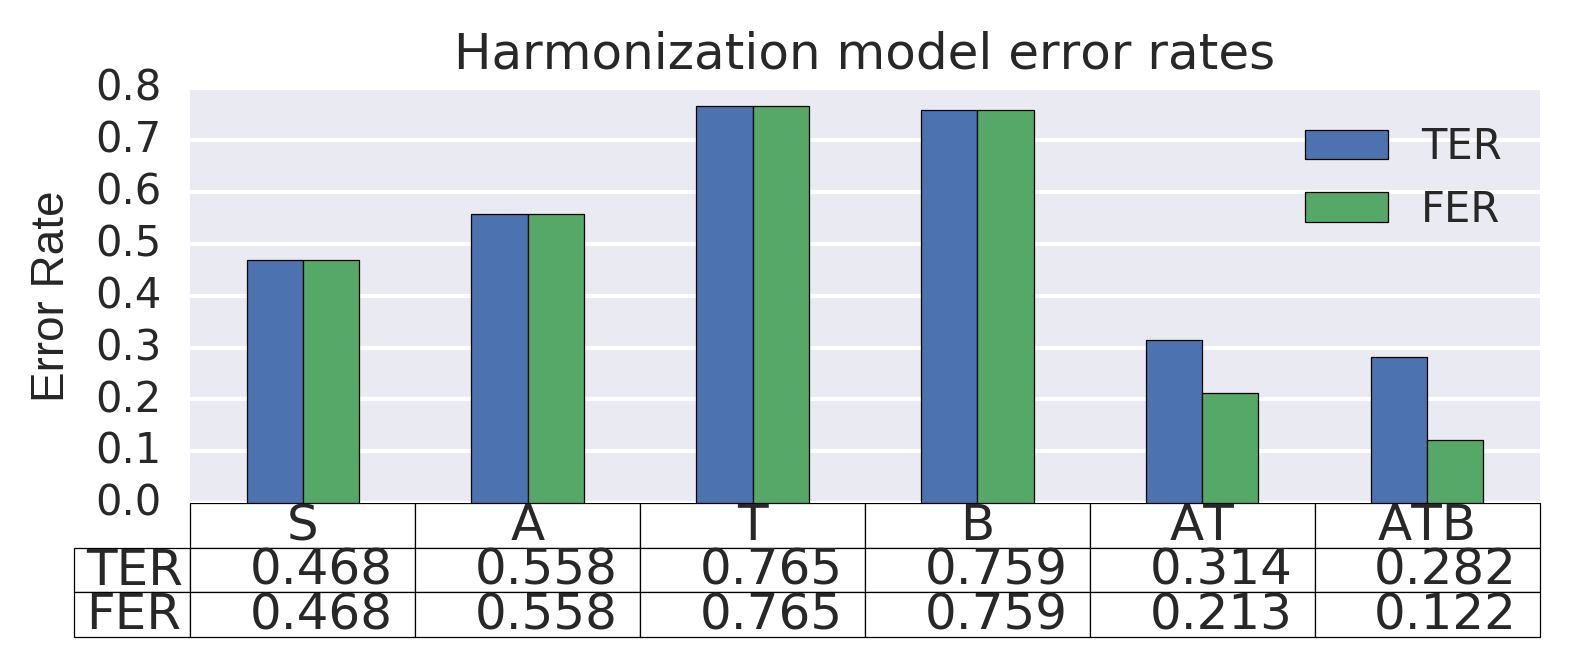
\includegraphics[width=1.0\linewidth]{harmonization-results.png}
  \caption{harmonization-Results}
  \label{fig:harmonization-results}
\end{figure}

\subsection{``Bachifying'' other music}

In addition to being able to harmonize Bach chorales, we found that BachBot was capable
of generating Baroque acompanyments to a variety of pieces. \cref{fig:harm-happy-birthday}
shows BachBot's proposed ATB harmonization for happy birthday\mynote{cite? public domain}
and \cref{fig:harm-twinkle-twinkle} for twinkle twinkle little star\mynote{cite?}.

\begin{figure}[htpb]
  \centering
  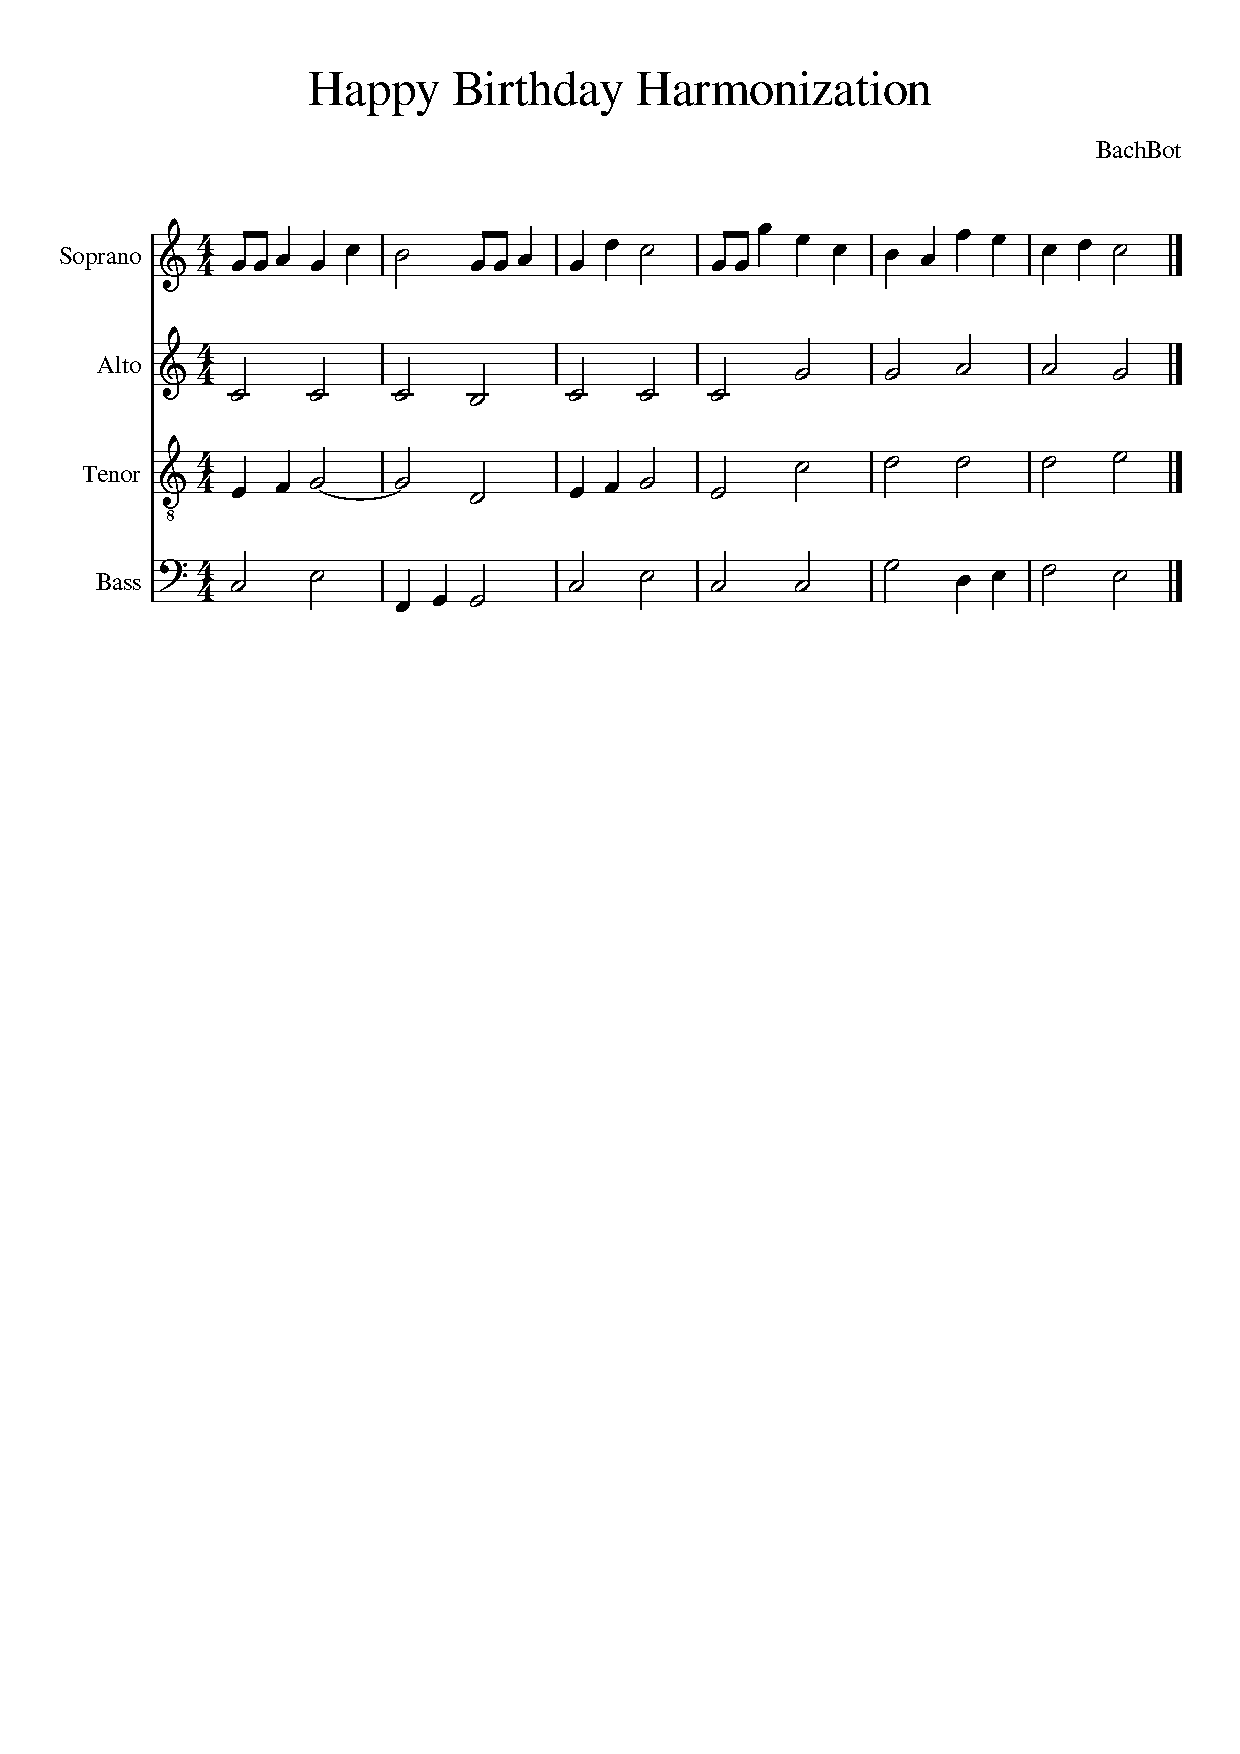
\includegraphics[trim={0 19cm 0 3.7cm},clip,width=0.9\linewidth]{happy-birthday-score.pdf}
  \caption{Happy birthday soprano melody, ATB harmonized by BachBot}
  \label{fig:harm-happy-birthday}
\end{figure}

\begin{figure}[htpb]
  \centering
  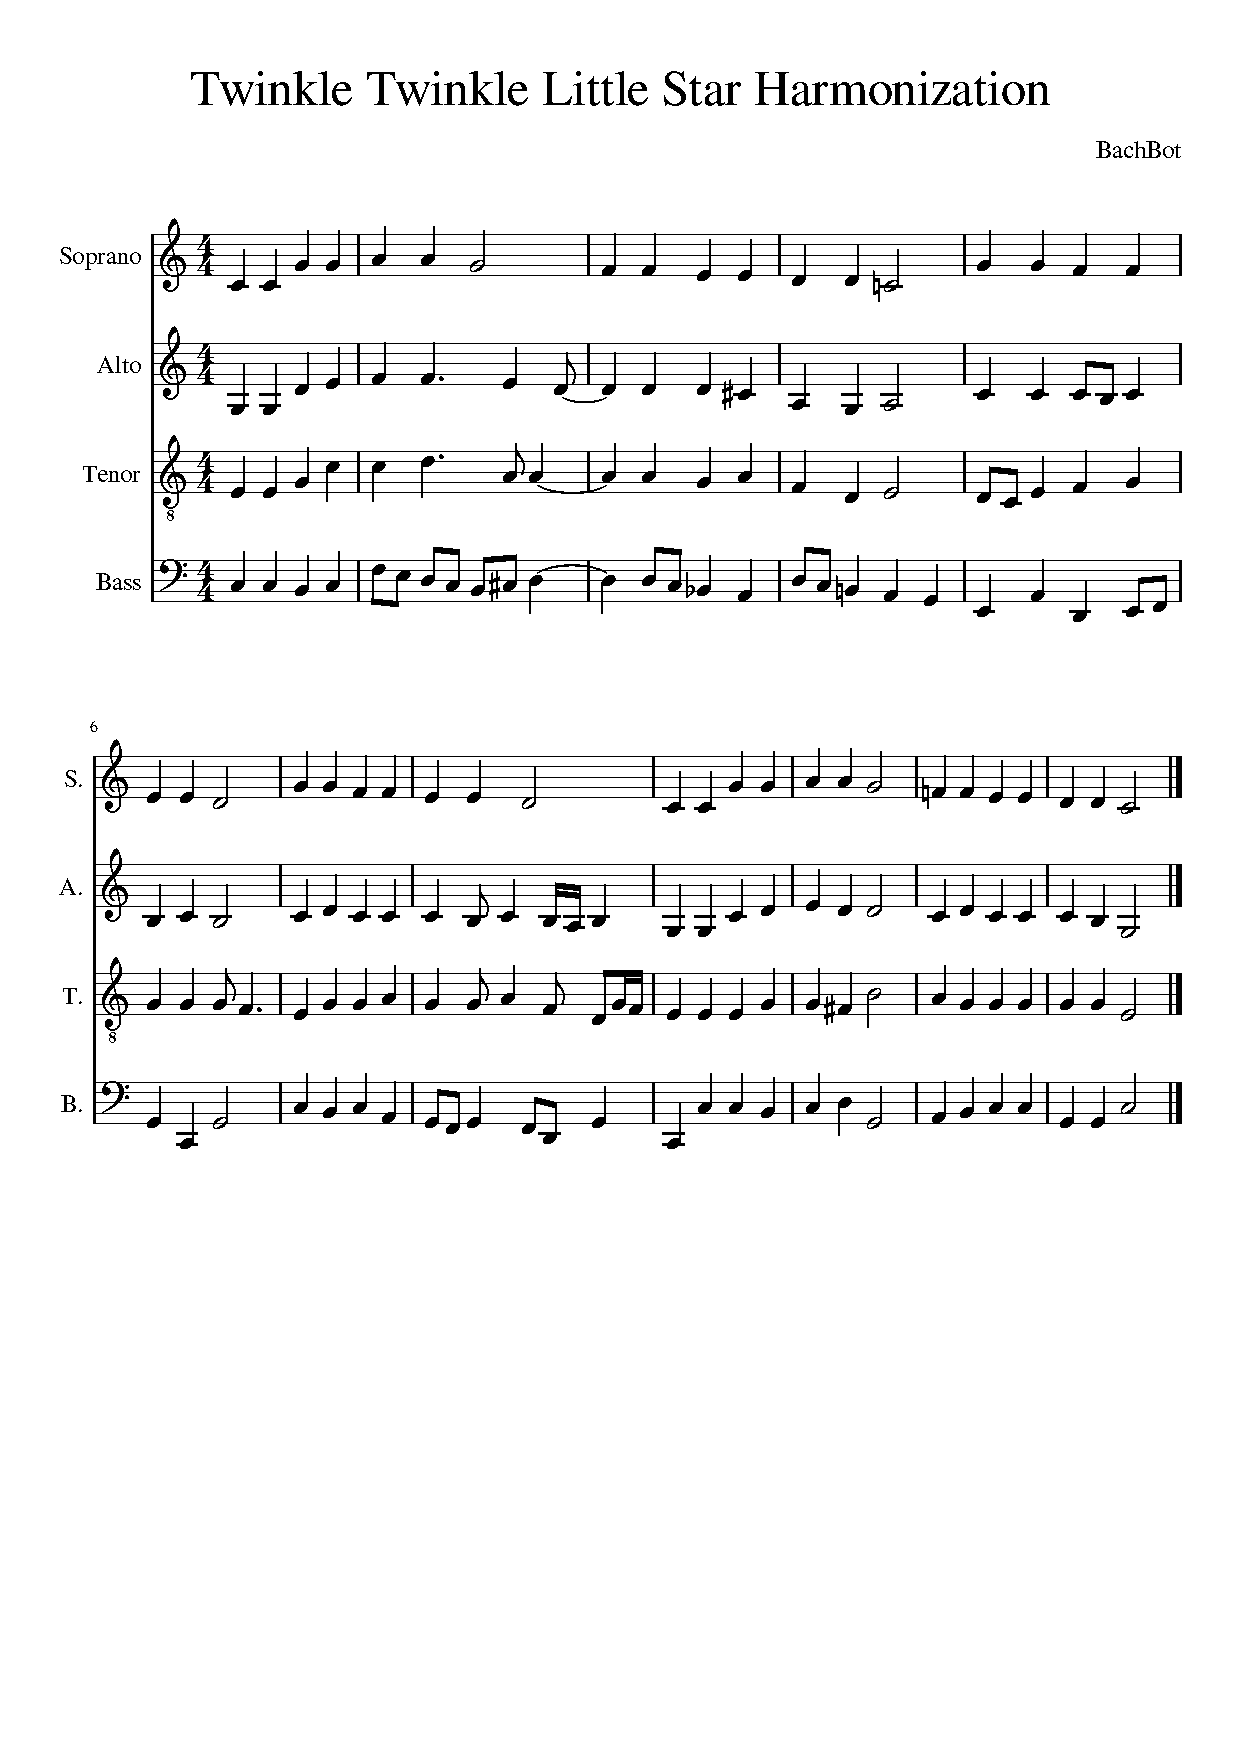
\includegraphics[trim={0 10cm 0 3.7cm},clip,width=0.9\linewidth]{twinkle-twinkle-score.pdf}
  \caption{Twinkle-twinkle soprano melody, ATB harmonized by BachBot}
  \label{fig:harm-twinkle-twinkle}
\end{figure}

\mynote{EXPERIMENT: Given the head, fill in the rest.}
